\section{Sperren}
\label{Sperren}

Betrachten Sie Ablauf \ref{ser_schedule1} aus Aufgabe \ref{serialisierbarkeit} und wenden darauf ein dynamisches Sperrkonzept an, indem Sie für jedes genutzte Datenobjekt je nach Bedarf S- bzw. X-Sperren anfordern und diese bis zum Ende der anfordernden Transaktion halten. Führen Sie dazu eine Sperrtabelle für jedes Datenobjekt. Wie verändert sich der Ablauf? Wurde durch die Sperren Serialisierbarkeit erreicht?

Hinweis: Sobald eine Transaktion eine angeforderte Sperre nicht bekommt, ist sie blockiert. Das bedeutet, sie kann die Operation, für die sie die Sperre angefordert hat, und alle folgenden Operationen solange nicht ausführen, bis sie diese Sperre bekommt. Andere Transaktionen des Ablaufs hingegen können weiterlaufen und mit einem commit enden, sobald sie alle ihre Operationen ausgeführt haben. In diesem Moment werden die von ihnen gehaltenen Sperren freigegeben, so dass Sperranforderungen anderer Transaktionen bedient werden können. Dadurch wird deren Blockade aufgehoben, so dass auch diese fortgeführt werden können. Sind alle beteiligten Transaktionen eines Ablaufs (die noch nicht beendet sind) blockiert, spricht man von einer Verklemmung (Deadlock). In diesem Fall ist der Ablauf nicht serialisierbar.

\beamertxt{\pagebreak}
Verwenden Sie folgende Notation:

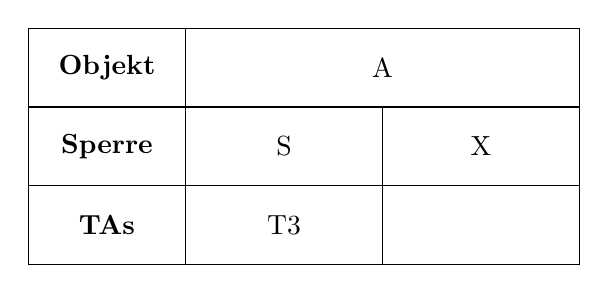
\begin{tikzpicture}
	\draw (0, 1) -- (7, 1);
	\draw (0, 2) -- (7, 2);
	\draw (2, 0) -- (2, 3);
	\draw (4.5, 0) -- (4.5, 2);
	\draw (0, 0) rectangle+(7, 3);

	\node at (1, 2.5) {\textbf{Objekt}};
	\node at (1, 1.5) {\textbf{Sperre}};
	\node at (1, 0.5) {\textbf{TAs}};

	\node at (4.5, 2.5) {A};
	\node at (3.25, 1.5) {S};
	\node at (5.75, 1.5) {X};

	\node at (3.25, 0.5) {T3};
\end{tikzpicture}

Dies bedeutet: T3 hält eine Shared-Sperre auf Objekt A. Wenn eine Transaktion T endet, müssen die Sperrtabellen für die Objekte neu gezeichnet werden, auf denen T Sperren gehalten hat.

\begin{beamerText}
 Ablauf: $r_2[B]$, $w_2[B]$, $r_1[A]$, $r_3[A]$, $r_3[B]$, $w_1[A]$, $w_3[A]$, $c_1$, $c_2$, $c_3$
\end{beamerText}
\begin{solution}
Der gegebene Ablauf ist: $r_2[B]$, $w_2[B]$, $r_1[A]$, $r_3[A]$, $r_3[B]$, $w_1[A]$, $w_3[A]$, $c_1$, $c_2$, $c_3$. Durch das Sperrkonzept ergibt sich folgender Ablauf:

\begin{enumerate}[1.]

	\item $T_2$ bekommt S-Sperre für B, anschließend wird diese in eine X-Sperre für B umgewandelt. $T_1$ und anschließend $T_3$ bekommen S-Sperre für A. $T_3$ fordert S-Sperre für B an und wird blockiert: $r_2[B]$, $w_2[B]$, $r_1[A]$, $r_3[A]$, \textcolor{red}{$r_3[B]$}, $\ldots$

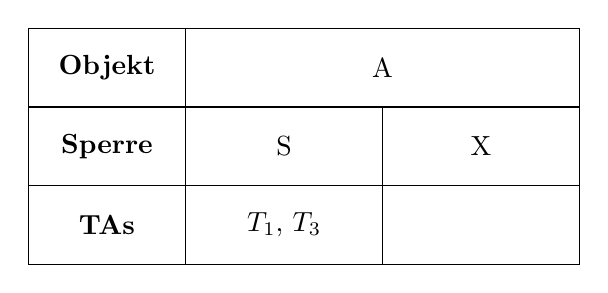
\begin{tikzpicture}
	\draw (0, 1) -- (7, 1);
	\draw (0, 2) -- (7, 2);
	\draw (2, 0) -- (2, 3);
	\draw (4.5, 0) -- (4.5, 2);
	\draw (0, 0) rectangle+(7, 3);

	\node at (1, 2.5) {\textbf{Objekt}};
	\node at (1, 1.5) {\textbf{Sperre}};
	\node at (1, 0.5) {\textbf{TAs}};

	\node at (4.5, 2.5) {A};
	\node at (3.25, 1.5) {S};
	\node at (5.75, 1.5) {X};

	\node at (3.25, 0.5) {$T_1$, $T_3$};
\end{tikzpicture}
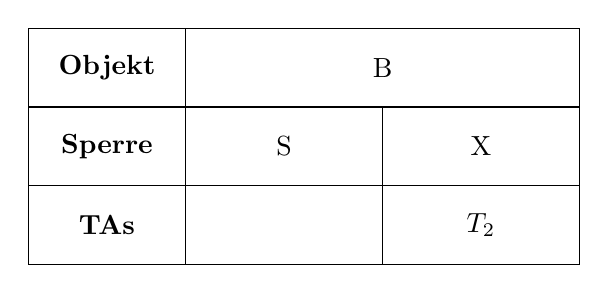
\begin{tikzpicture}
	\draw (0, 1) -- (7, 1);
	\draw (0, 2) -- (7, 2);
	\draw (2, 0) -- (2, 3);
	\draw (4.5, 0) -- (4.5, 2);
	\draw (0, 0) rectangle+(7, 3);

	\node at (1, 2.5) {\textbf{Objekt}};
	\node at (1, 1.5) {\textbf{Sperre}};
	\node at (1, 0.5) {\textbf{TAs}};

	\node at (4.5, 2.5) {B};
	\node at (3.25, 1.5) {S};
	\node at (5.75, 1.5) {X};

	\node at (3.25, 0.5) {};
	\node at (5.75, 0.5) {$T_2$};
\end{tikzpicture}

	\item $T_1$ fordert X-Sperre für A an und wird ebenfalls blockiert. Das bedeutet, es kann nur noch $T_2$ ausgeführt werden. $T_2$ hat aber bereits alle Operationen ausgeführt, d.\,h.\ sie kann mit commit enden und ihre Sperren werden wieder freigegeben: \textcolor{red}{$r_3[B]$}, \textcolor{red}{$w_1[A]$}, $w_3[A]$, $c_1$, $c_2$, $c_3$.

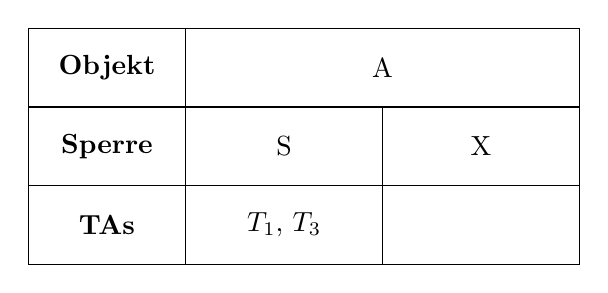
\begin{tikzpicture}
	\draw (0, 1) -- (7, 1);
	\draw (0, 2) -- (7, 2);
	\draw (2, 0) -- (2, 3);
	\draw (4.5, 0) -- (4.5, 2);
	\draw (0, 0) rectangle+(7, 3);

	\node at (1, 2.5) {\textbf{Objekt}};
	\node at (1, 1.5) {\textbf{Sperre}};
	\node at (1, 0.5) {\textbf{TAs}};

	\node at (4.5, 2.5) {A};
	\node at (3.25, 1.5) {S};
	\node at (5.75, 1.5) {X};

	\node at (3.25, 0.5) {$T_1$, $T_3$};
\end{tikzpicture}
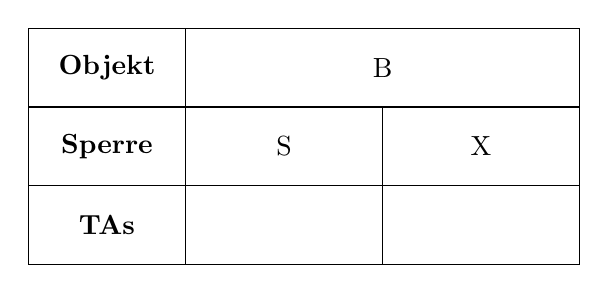
\begin{tikzpicture}
	\draw (0, 1) -- (7, 1);
	\draw (0, 2) -- (7, 2);
	\draw (2, 0) -- (2, 3);
	\draw (4.5, 0) -- (4.5, 2);
	\draw (0, 0) rectangle+(7, 3);

	\node at (1, 2.5) {\textbf{Objekt}};
	\node at (1, 1.5) {\textbf{Sperre}};
	\node at (1, 0.5) {\textbf{TAs}};

	\node at (4.5, 2.5) {B};
	\node at (3.25, 1.5) {S};
	\node at (5.75, 1.5) {X};
\end{tikzpicture}

	\item Jetzt bekommt $T_3$ die S-Sperre für B, $T_1$ ist weiterhin blockiert. Anschließend fordert $T_3$ eine X-Sperre für A an und ist wieder blockiert. Damit befindet sich der Ablauf in einer Verklemmung: $r_3[B]$, \textcolor{red}{$w_1[A]$}, \textcolor{red}{$w_3[A]$}, $c_1$, $c_3$.

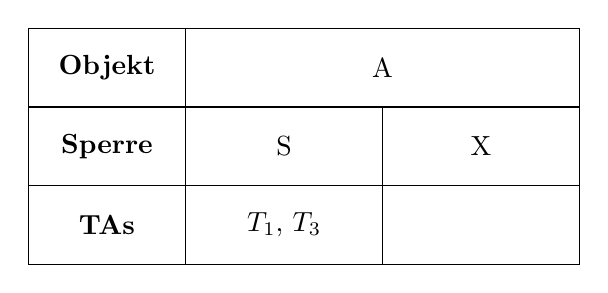
\begin{tikzpicture}
	\draw (0, 1) -- (7, 1);
	\draw (0, 2) -- (7, 2);
	\draw (2, 0) -- (2, 3);
	\draw (4.5, 0) -- (4.5, 2);
	\draw (0, 0) rectangle+(7, 3);

	\node at (1, 2.5) {\textbf{Objekt}};
	\node at (1, 1.5) {\textbf{Sperre}};
	\node at (1, 0.5) {\textbf{TAs}};

	\node at (4.5, 2.5) {A};
	\node at (3.25, 1.5) {S};
	\node at (5.75, 1.5) {X};

	\node at (3.25, 0.5) {$T_1$, $T_3$};
\end{tikzpicture}
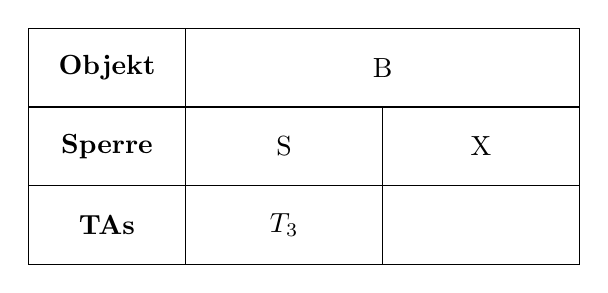
\begin{tikzpicture}
	\draw (0, 1) -- (7, 1);
	\draw (0, 2) -- (7, 2);
	\draw (2, 0) -- (2, 3);
	\draw (4.5, 0) -- (4.5, 2);
	\draw (0, 0) rectangle+(7, 3);

	\node at (1, 2.5) {\textbf{Objekt}};
	\node at (1, 1.5) {\textbf{Sperre}};
	\node at (1, 0.5) {\textbf{TAs}};

	\node at (4.5, 2.5) {B};
	\node at (3.25, 1.5) {S};
	\node at (5.75, 1.5) {X};

	\node at (3.25, 0.5) {$T_3$};
\end{tikzpicture}

Um den Deadlock aufzuheben, müsste nun eine der beiden Transaktionen abgebrochen werden.
Hierdurch werden die Sperren dieser Transaktion freigegeben, so dass die andere weiterlaufen kann.

\end{enumerate}

\end{solution}


\subsection*{Zusatzfrage}

Die Ausführung eines nicht serialisierbaren Ablaufs mit Sperren führt nicht immer zur Verklemmung.
Sind in diesem Fall der ursprüngliche und der mit Sperren realisierte Ablauf äquivalent?

\begin{solution}
Die Antwort ist: Nein, denn ein sperrbasierter Ablauf ohne Verklemmung ist immer serialisierbar und ein serialisierbarer und ein nicht-serialisierbarer Ablauf können nicht äquivalent sein.

Ein Beispiel für einen solchen Ablauf ist folgender: \\
$r_3[A], w_3[A], r_1[A], r_1[B], r_2[B], w_2[B], w_3[B], c_1, c_2, c_3$

Der zugehörige Abhängigkeitsgraph enthält zwei Zyklen und sieht so aus:

\begin{tikzpicture}
	\node (T3) at (0,0) {$T_3$};
	\node (T1) [below of = T3, yshift = -0.5cm, xshift=-2cm] {$T_1$};
	\node (T2) [below of = T3, yshift = -0.5cm, xshift=+2cm] {$T_2$};
	\node [right of =T3, xshift=0.3cm, yshift=-0.5cm] {B};
	\node [below of = T3, xshift=-0.9cm] {B};
	\node [left of = T3, xshift=-0.25cm, yshift=-0.3cm] {A};
	\node [below of = T3, yshift=-0.2cm] {B};

	\draw[-triangle 60] ($(T1.east)$) -- ($(T2.west)$);
	\draw[-triangle 60] (T1) -- ($(T3.south) + (-0.2, 0.1)$);
	\draw[-triangle 60] (T2) -- ($(T3.south) + (0.3, 0.1)$);
	\draw[-triangle 60] ($(T3.west)$) -- ($(T1.north) + (-0,0)$);
\end{tikzpicture}

Wendet man ein dynamisches Sperrkonzept an, sieht der Ablauf folgendermaßen aus: $T_1$ wartet auf $T_3$, $T_3$ wartet auf $T_2$, $T_2$ läuft durch, $T_3$ läuft durch, $T_1$ läuft durch.
\end{solution}
